\documentclass{mprop}
\usepackage{graphicx}
\usepackage{hyperref}
\usepackage{url}
\usepackage{amsmath}
\usepackage{caption}
% alternative font if you prefer
%\usepackage{times}

% for alternative page numbering use the following package
% and see documentation for commands
%\usepackage{fancyheadings}


% other potentially useful packages
\usepackage{epigraph}
%\uspackage{amssymb,amsmath}
%\usepackage{fancyvrb}
%\usepackage[final]{pdfpages}

% Inspirational Quote type setting
\makeatletter
\newenvironment{chapquote}[2][2em]
  {\setlength{\@tempdima}{#1}%
   \def\chapquote@author{#2}%
   \parshape 1 \@tempdima \dimexpr\textwidth-2\@tempdima\relax%
   \itshape}
  {\par\normalfont\hfill--\ \chapquote@author\hspace*{\@tempdima}\par\bigskip}
\makeatother

\begin{document}

%%%%%%%%%%%%%%%%%%%%%%%%%%%%%%%%%%%%%%%%%%%%%%%%%%%%%%%%%%%%%%%%%%%
\title{Securing and Integrating the IoT with a Smart Home Router}
\author{Fergus W. Leahy}
\date{16/12/2013}
\maketitle
%%%%%%%%%%%%%%%%%%%%%%%%%%%%%%%%%%%%%%%%%%%%%%%%%%%%%%%%%%%%%%%%%%%

%%%%%%%%%%%%%%%%%%%%%%%%%%%%%%%%%%%%%%%%%%%%%%%%%%%%%%%%%%%%%%%%%%%
\tableofcontents
\newpage
%%%%%%%%%%%%%%%%%%%%%%%%%%%%%%%%%%%%%%%%%%%%%%%%%%%%%%%%%%%%%%%%%%%

%%%%%%%%%%%%%%%%%%%%%%%%%%%%%%%%%%%%%%%%%%%%%%%%%%%%%%%%%%%%%%%%%%%
\section{Introduction}
\label{sec:introduction}

\begin{chapquote}{Mark Weiser, \textit{The Computer for the Twenty-First Century, 1991}}
    ``The most profound technologies are those that disappear. They weave themselves into the fabric of everyday life until they are indistinguishable from it.''
\end{chapquote}

The modern home is becoming increasingly filled with a variety of \textit{connected} devices (laptops, tablets, phones, set-top boxes etc.), providing a myriad of different services to users within the home. On top of this, with the introduction of smart phones and wearable devices, we too are starting to carry around our own personal network of devices everywhere we go, brushing past many others in our daily lives at home, work and on the street. Although all connected to the Internet, these devices are often encapsulated within their own environment and ecosystem, unable to interconnect, creating a fractured and often complex user experience. 

Making matters more interesting, the Internet of Things paradigm is once again becoming a field of great interest due to the advent of cheap, low-power wireless embedded devices \cite{2013IoT}. However, not much consideration has been made for how these Things should be integrated into the existing home network, with many approaches opting to simply bridge the device to the cloud (\cite{SmartThings}, \cite{Twine}, \cite{IETF_CORE}), with obvious concerns for security, privacy and up-time.

As these devices enter our homes and pockets, bringing with them their own ecosystems, the user is faced with the increasingly difficult burden of managing them and their ecosystems \cite{brundell2011w}, \cite{brown2013multinet}. Due to the sheer number and diversity of these devices, many of which will provide overlapping services and functionality, problems arise with respect to how these devices cooperate, as well as how to ensure that the user's network and information stays secure against new and unanticipated threats.

In order for these multiple layered networks of devices to truly fade away into the fabric of our everyday lives, a platform and relevant protocols need to be engineered to not only support this heterogeneous network securely, but also aid the user in managing both the network and the privacy of their information.

The Homework home router platform was created to address these issues. Rather than assume every user is a network administrator, the project investigated the needs and abilities of the average user in order to propose the future of home networking, re-inventing the protocols, models and architectures to truly suit the home environment. This re-invention of the home router allows a user to easily install, manage and use their home network, without the need of a Cisco qualification.

In regards to the Internet of Things development, previous work demonstrated that it was in need of a suitable protocol in order to meet the specific needs of a network of Things \cite{KNoT}. Thus, a new protocol was designed and implemented, which could not only run on the most constrained battery-powered devices (8MHz), but it could also efficiently scale to support hundreds of Things within the same network.

%TODO: WRITE MORE LINKY LINKY

%briefly explain the context of the project problem

%%%%%%%%%%%%%%%%%%%%%%%%%%%%%%%%%%%%%%%%%%%%%%%%%%%%%%%%%%%%%%%%%%%

\section{Statement of Problem}
\label{sec:statement_of_problem}
Whilst there have been many attempts, both past and recent, to create the perfect Internet of Things network for the home, all still exhibit several issues. This section will first present a typical user scenario to provide a context for this problem, then discuss several of the issues found in existing work, both our previous work and others', which provide the motivation for this project.

\subsection{A Scenario} % (fold)
\label{sub:scenario}
In order to establish the context of the problem, a typical user scenario has been created to demonstrate a typical novice user purchasing a new Thing and attempting to integrate it into their network securely with minimal knowledge and effort.

\textit{Bob buys a new Thing, a motion sensor, from a shop and brings it home. He wants to connect it to his currently existing home network. To do so, Bob turns on the Thing and presses the connect button on both the Thing and his home router. Using his tablet/PC Bob is able to view the newly available Things in the network that he can connect to, in which he can see his new Thing. Bob is able to view various information about the Thing, including it's type, manufacturer, functions etc. Bob selects the Thing he wants to connect to the network and within a minute the new thing is now part of the network and he can then customise how he wants to use it in the network.}

\subsection{The Problem} % (fold)
\label{sub:the_problem}
The Internet of Things protocol created in \cite{KNoT} proved to be a successful proof-of-concept; however, in order for it to be considered for deployment and integration into existing homes, two main issues need to first be addressed.

\subsubsection{Security} % (fold)
\label{ssub:security}

The initial design of the IoT protocol didn't consider security due to time constraints; however, because not only can such rich and sensitive data can be gathered about the user and their home from Things, but the closed loop of control can be affected by injection; therefore it becomes extremely important to not only protect the data from unauthorised access, but also protect the network itself. 
Presented below is a summary of the typical attacks targeted towards WSNs, and in this case an IoT.
\begin{enumerate}
  \item \textbf{Eavesdropping} - An attacker observes the unencrypted traffic between the various devices in the network, and uses this information for illegitimate purposes. This needs to be prevented due to the richness, coverage and sensitivity of the data captured within an IoT, which could be used to perform serious physical attacks, spying, as well as have other serious consequences. Therefore, it's necessary to encrypt all traffic where possible, so that only legitimate participants may observe the information traversing the network.
  \item \textbf{Unsanctioned participants} - An attacker infiltrates the network masquerading as a legitimate participant, enabling it to spoof traffic, such as events and commands, as well as observe other traffic. Such an attack would enable an attacker to spy on and manipulate the network of Things, which could lead to various damaging consequences, ranging from energy waste, to more serious home security issues such security locks being disabled enabling other possible crimes.
  \item \textbf{Node capture} - Due to the placement of Things, sometimes outwith the protective confines of a home or building, they can become vulnerable to an attacker capturing them. Once captured, it may be possible to extract encryption keys, illegally modify the functionality and also replace nodes with maliciously modified ones.
  \item \textbf{Denial of service} - 
\end{enumerate}

Demonstrated in the scenario, a user may want to purchase any kind of compatible Thing from a shop and then want bring it into their home network with minimal effort. The Thing itself would have no prior knowledge of the network and needs a secure mechanism to enter the network without compromising the rest of the network or exposing its own data to unauthorised users. 
% subsubsection security (end)

\subsubsection{Integration} % (fold)
\label{ssub:integration}

The current implementation exists as a standalone library with several demo applications. Integration of the IoT protocol into a user-friendly platform is necessary to harness the full power of a network of Things. The integrated platform would then be able to discover and connect to available Things, subscribe and log events from the sensors, and using user customised rules, use automata to detect if these rules are met and then perform actions by publishing commands to actuators in the network.
% subsubsection integration (end)

\subsection{Intranet of Things vs Internet of Things} % (fold)
\label{sub:intranet_of_things}

As described earlier in section \ref{sec:introduction}, many previous deployments of Internet of Things networks have taken a cloud first approach \cite{SmartThings, Twine}. Whilst this yields certain benefits, such as easy external access and integration with other services \cite{IFTTT, Xively}, it also poses several questions regards data security, privacy and up-time. For this project, the focus will be on developing a home first platform, in which all Things communication will be kept local, with no cloud processing involved; thus a more suitable name, the Intranet of Things, will be used. 
% subsection intranet_of_things (end)

% subsection the_problem (end)
\subsection{Project Outcomes} % (fold)
\label{sub:project_outcomes}

Outcomes of the project:
\begin{itemize}
  \item[-] An extended IoT protocol with sufficient security to prevent eavesdropping and unsanctioned devices.
  \item[-] An Extended home information platform (Homework), with the IoT controller role implemented, enabling capturing of IoT events from sensors and creation of commands for actuators.
  \item[-] Use of Homework's automata to implement closed loop control of Things in the home, subscribing to sensor events, processing rules and publishing to actuators to perform actions.
\end{itemize}
% subsection subsection_name (end)

% clearly state the problem to be addressed in your forthcoming project. Explain why it would be worthwhile to solve this problem.

\subsection{Structure} % (fold)
\label{sub:structure}
The rest of this proposal is structured in the following way. Section 3 surveys previous work on the field of wireless sensor networks security, home networks and Internet of Things systems and protocols. Section 4 takes what has been learnt from the literature survey and proposes a solution to solve the problem described above. Lastly, section 5 discusses the work plan outlined for the implementation and evaluation part of the project, for the second half of the year.
% subsection structure (end)

%%%%%%%%%%%%%%%%%%%%%%%%%%%%%%%%%%%%%%%%%%%%%%%%%%%%%%%%%%%%%%%%%%%

\section{Literature Review}
This section discusses previous work on Internet of Things protocols, WSN security and home networking which provides the motivation and possibly aids in solving the previously mentioned issues.

\subsection{State-of-the-art IoT Protocols} % (fold)
\label{sub:state_of_the_art_iot_protocols}
Over the last 20 years, the Internet of Things has developed and evolved continuously, from 20 years ago where it was the concept of using barcodes, and later RFID\cite{K.Ashton}, to track items in a warehouse, to today where our home appliances are filled with ``smart'' electronics, able to sense, react and notify the user of events, such as the washing machine finishing a load. Whilst the Internet of Things has been around for quite some time, under various guises, it's yet to become commercially successful and see wide-spread deployment; Many believe that 2013 is the year that the Internet of Things will truly take off and become ubiquitous in our daily lives\cite{2013IoT}.

The rest of this section will discuss the various different attempts made to create Internet of Things networks in the home.

\subsubsection{Smart Things} % (fold)
\label{ssub:smart_things}
Launched in 2012, the SmartThings platform aims to allow the user to turn any ordinary object in the home into a ``Smart'' object by giving it the ability to connect to the Internet. The platform consists of a central hub connected to the Internet, containing a low-power Zigbee radio, from which it connects to an array of SmartThings accessories as well as many pre-existing third party Zigbee devices. Some of these accessories include motion detectors, moisture sensors, vibration detectors, power-plug switches as well as many others. The user can then view and interact with their Smart Things through the cloud service via an Internet-connected PC or a smartphone, allowing them to either control the devices directly or set-up rules/schedules for devices.

\begin{figure}[h!]
\centering
    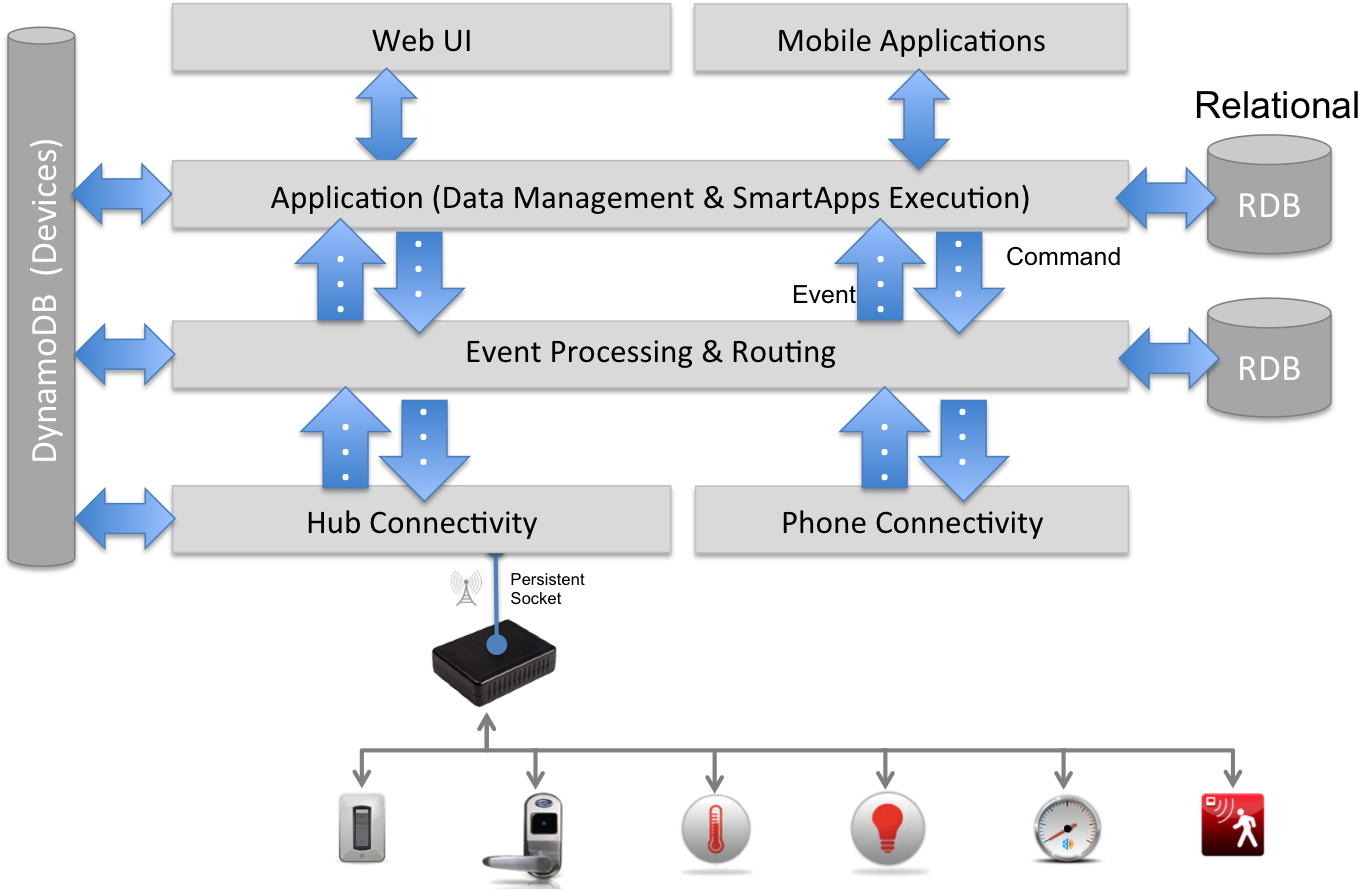
\includegraphics[scale=0.4]{images/smartThingsCloudFirstDiagram.png}
    \caption[]{Smart Things - Cloud approach\footnotemark}
    \label{fig:cloud}
\end{figure}
\footnotetext{Image from Smart Things developer support: \url{https://support.smartthings.com/entries/21603009-Device-Types-Capabilities-Attributes}}

As shown in figure \ref{fig:cloud}, Smart Things takes a cloud approach, offloading all processing to the cloud, leaving the hub to just act as a gateway and translator between the Things and the cloud. By utilising the cloud in this way, it enables the hub to be a very simple and low-power device, reducing both the purchasing and running costs for the user. It also allows the user to access their network of Things from anywhere, at any time, which would otherwise be difficult to do in a local approach. 

However, the cloud approach also has several drawbacks. By offloading the entire processing needs of the network, as show above, the network of Things becomes vulnerable to failure if either the network fails or is unresponsive, or if the cloud service fails or goes down for maintenance. Another issue is the privacy of the user's data; How safe is the data in the cloud and how secure are the services they make available for users to interact with their devices with. There have been many examples of online services that have been attacked, leaking user data and/or shutting down for extended periods of time \cite{Playstation, Amazon, Google}.

Talk about integration of two home networks.


% Currently, there is no information on how the underlying protocol for connecting the SmartThings to the hub works, but at the time of writing, the current implementation uses a ``cloud first'' approach. This means that rather than the hub wiring all devices together based on the rules and schedules set up by the user, all the intelligence of the network is being handled in the cloud. This brings about the problem of Internet connectivity, with two points of failure, either the user or the cloud. From the user's standpoint, an Internet connection might not be available where the hub is located, or the user could have a faulty, slow or non-permanent connection, which renders all the SmartThings devices into dumb devices. In contrast to this, because of the reliance on the cloud, if the cloud service provider experiences downtime then all SmartThings users devices become dumb devices. In cases where these devices are used for security and safety, dire consequences could result.
% subsubsection smart_things (end)

\subsubsection{CoRE CoAP HIP-DEX} % (fold)
\label{ssub:core_coap}

% subsubsection core_coap (end)
\subsubsection{KNoT} % (fold)
\label{ssub:knot}

% subsubsection knot (end)
% subsection state_of_the_art_iot_protocols (end)

\subsection{Home networking} % (fold)
\label{sub:homework_smart_home_router}
\textbf{Discuss Homework router and cache db}
% subsection homework_smart_home_router (end)

%%%%%%%%%
\subsection{WSN Security - Symmetric Cryptography} % (fold)
\label{sub:tinysec_minisec_contikisec}
Substantial research has been carried out to secure WSNs, to ensure data within the network can't be compromised, enabling attackers to eavesdrop and/or masquerade as sanctioned participants, and introduce bogus data that can affect the control loop activity, or leak sensitive data.

Symmetric key cryptography is a class of cryptographic algorithms which enable two participants to exchange data in secret over a public channel using a shared key, known by both participants. Both encryption and decryption use the same key. One of the key benefits to symmetric algorithms is that it's relatively inexpensive, both in time and space, to encrypt and decrypt data, which makes this ideal for use in a WSN where resources are extremely constrained.

Symmetric algorithms fall into two main categories, stream based ciphers, where data is encrypted by combining it with a pseudorandom data stream (one time pad), and block based ciphers, where data is segmented into blocks and operated on by a set of functions, often with the previous cipher block feeding into the next input. 

In the case of WSN, block based ciphers have seen exclusive use. However, one issue with a block based cipher is that if two identical blocks are encrypted, both will return equal encrypted blocks, thus a passive adversary could extract partial information about the plaintext sent (semantic security). To solve this and maintain semantic security, an additional security primitive, an initialisation vector, can be used to ensure that this cannot occur. An initialisation vector provides a unique value which is used in the encryption of the first block, ensuring no two identical blocks return the same cipher text block; after the first block, the initialisation vector becomes the previous ciphertext block.

The rest of this section discusses several attempts to secure WSNs using symmetric key cryptography for both the TinyOS and Contiki WSN operating systems, mentioning both the benefits and some drawbacks apparent in each. 


\subsubsection{TinySec} % (fold)
\label{ssub:tinysec}
TinySec is a fully functional symmetric security link layer component created for the wireless sensor network operating system, TinyOS. It was the first fully implemented solution for WSNs and was created to address the security worries of running a WSN and transmitting private sensor data in the clear. Unlike conventional security protocol implementations which can afford significant time and space overheads, such as 16-32 bytes for security per packet, WSN typically run on extremely constrained devices with packet sizes of just 30 bytes, making those implementations impossible/extremely expensive to run.

To resolve this, TinySec took a balanced approach making a compromise between the level of security, packet overhead and resource requirements. The end result proved that it's possible to secure a WSN efficiently entirely in software, without the need for additional hardware. 

Communication between nodes, not just nodes-to-base-station, in WSNs is often quite important, allowing nodes to not only redirect other's traffic along routes but also consolidate duplicate packets from multiple nodes about the same event, saving the overall network from wasting power receiving and transmitting the extra packets; tinySec chose to engineer in security at the link layer, allowing these mechanisms to perform without alteration. The security goals of TinySec aimed to enable access control, whereby only authorised participants may participate in the network, with unauthorised messages easy to spot and reject; ensure message integrity, so that authorised messages can't be illegally altered by a man-in-the-middle without the receiver noticing; and ensure confidentiality, to ensure information is kept secret from unauthorised eavesdroppers. 

The TinySec implementation uses Cipher Block Chaining with an initialisation vector (IV), together these achieve semantic security, therefore ensuring that encrypting the same plain text twice returns a different cipher text each time. So that the receiving end knows how to begin decryption of the data, the IV must be sent in the clear along with the encrypted data. When using an IV, its length needs to be taken into consideration because repeats will occur when the number wraps, causing a security vulnerability. On unconstrained devices an IV is usually 8 or 16 bytes, however due to the packet size limitations of the wireless sensors used, a 8(2 byte counter) byte IV was chosen. In the IV, 6 bytes are made up of pre-existing fields to conserve space and ensure globally unique IVs in the network e.g. to nodes send the same data event and both happen to have the same counter value, but differ in source (src), so the IV is different, therefore preserving the security.

For ensuring authenticity and integrity of messages, TinySec uses Cipher Block Chaining Message Authentication Codes (CBC-MAC) of 4 bytes in length. Similar to a CRC, CBC-MAC runs over the data and produces a 4 byte MAC which is appended to the packet. If a message was to be altered, the attacker has a 1 in $2^{32}$ of blindly forging a valid MAC. In a WSN with a limited send rate of 19.2Kb/s it would take over 20 months to send enough packets to possibly succeed in forging a MAC. In the case of attack, a receive heuristic could be used to detect multiple failed MAC transmissions at a nearby node, triggering an alert to the rest of the network.

Whilst TinySec can secure a WSN against eavesdropping and forged messages, it has two significant drawbacks. Firstly, in regards to key distribution, encryption and authentication keys need to be loaded to the nodes prior to deployment. This can cause issues when the shared keys need to be changed, such as when they are compromised, as all nodes in the network will need the new key. This can be especially difficult post-deployment, simply due to the number of nodes and often embedded and/or difficult to reach locations. Secondly, if a node in the network is compromised, because the authentication key is a network wide shared key, the illegitimate node can pretend to be any other node in the network, making it difficult to protect, never mind counter against.
% subsubsection tinysec (end)

\subsubsection{MiniSec} % (fold)
\label{ssub:minisec}
MiniSec was created to tackle several problems apparent in the then current WSN security protocols, TinySec and Zigbee \cite{MiniSec}. The pre-cursor to MiniSec, TinySec, received much attention and use due to its power and resource efficient security implementation, but because of limited authentication and lack of replay prevention, the overall security provided was deemed insufficient to protect a WSN. A commercial alternative, Zigbee, exhibits significantly higher security, but does so at the cost of higher energy consumption. MiniSec was designed to find the middle-ground between the two, increasing security whilst remaining energy efficient. 

In contrast to TinySec, for its encryption mode of operation, MiniSec uses Offset Code Book. Unlike cipher block chaining (CBC) which requires two passes to provide both encryption and authentication, OCB provides both in only one pass over the data. This one pass also performs faster that CBC's two passes and only requires one key for operation, thus making it more appropriate for a constrained device in terms of power and storage. 

MiniSec also differs from TinySec by reducing the size of the IV counter sent in a packet, yet managing to increase the size of the IV so that it wraps less often. This is achieved by storing some state about the IV counter locally and only transmitting the last n bits of it to the receiving node. This also requires some logic on both sides to manage the counter in the event of packet loss larger than the range of values stored in the last n bits sent, i.e. when $>2^n$ are lost. For MiniSec, the authors chose n = 3. Because of this, only 3 extra bits needed to be sent with a packet, instead of the 2 extra bytes in TinySec. However, this overhead could be removed altogether. The maximum default packet size in TinyOS is 29 bytes, therefore the 3 most significant bits in the packet-size byte aren't used and can instead be used to store the IV counter. Therefore the need for the extra byte to store those bits is eliminated.\footnote{The publicly available source code for MiniSec (\url{https://sparrow.ece.cmu.edu/group/minisec.html}) does not make use of this technique, instead it appends an additional byte, thus reducing the benefit of the proposed reduced packet-size state-based counter.}

Another improvement, is the use of the synchronised counter (also used as the IV) to prevent replay attacks. As each packet is received, the counter is incremented accordingly, thus if a packet arrives with a counter less than the one stored locally, it is dropped as one can determine it must be a replayed packet. 

% subsubsection minisec (end)

\subsubsection{ContikiSec} % (fold)
\label{ssub:contikisec}
Similar to TinySec\cite{TinySec} and MiniSec\cite{MiniSec}, ContikiSec \cite{ContikiSec} is an asymmetric cryptographic security network layer, however, it's built for the other significant WSN OS, Contiki, instead of TinyOS. The paper presents two main contributions; first, an extensive evaluation of several block-ciphers and modes-of-operation, comparing ROM/RAM sizes and timings; second, a modular asymmetric encryption network layer for Contiki, offering modes for encryption, authentication or encryption + authentication.

After comparing several block ciphers (AES, Skipjack, RC5, Triple-DES, Twofish and XTEA), AES was chosen for use in ContikiSec due to its good trade-off between resource consumption and security. This is in contrast to both TinySec and MiniSec, which chose to use Skipjack. At the respective times of publication of TinySec and MiniSec, Skipjack was deemed sufficiently secure by NIST until 2008. Similar to MiniSec, ContikiSec also uses offset codebook as its mode of operation, combining both encryption and authentication into one pass.
% subsubsection contikisec (end)
% subsection tinysec_minisec_contikisec (end)
%%%%%%%%%

\subsection{Key Distribution Problem} % (fold)
\label{sub:key_distribution_problem}

Whilst previous work has demonstrated it is feasible to secure a wireless sensor network against eavesdropping, unauthorised participants and replay attacks, the issue of key distribution still remains.
In the typical academic scenario, this may be a non-issue due to the expertise of the users. However, as described in the scenario in section \ref{sec:statement_of_problem}, the typical home user will only have a very basic knowledge, if any, of how to use and operate the devices, let alone configure and distribute network encryption keys on all of their Things. Therefore, it becomes necessary to investigate a method by which the keys for symmetric cryptography can be distributed, with minimal effort and knowledge required from the user.

\subsubsection{USB interface connectivity} % (fold)
\label{ssub:usb_interface_connectivity}
A simple method of distributing keys could be to force the user to plug the Thing into their PC or router, which would then automatically program the correct key into the device with minimal user interaction. Whilst this seems attractive at first, the main issue with this method is that it requires every Thing to have a USB port, plus the appropriate circuitry and logic to perform the programming. This not only increases the cost for the Things, as they now require additional components, but it can also increase the physical size and complexity of using them.
% subsubsection usb_interface_connectivity (end)

\subsubsection{Message-in-a-bottle} % (fold)
\label{ssub:message_in_a_bottle}
In an attempt to distribute session keys in a user friendly way, and without the use of physical interfaces or asymmetric cryptography, Message-in-a-bottle utilises several physical techniques to carry out a wireless keying mechanism resilient to typical WSN attack vectors \cite{MessageBottle}. To achieve this, a Faraday cage and RF jamming is used in combination with a wireless session key distribution protocol. 

To distribute the session key to a new uninitialised device, a user places the keying device and the new device entering the network into a Faraday cage\footnote{The authors used a steel pipe sealed at both ends.}. The keying device then wirelessly transmits keying information to the node inside the cage. Meanwhile outside the cage, a keying beacon jams the wireless frequency of the shielded devices, in an attempt to ensure no leakage happens due to imperfections in the cage. After the keying session has complete, signalled by the keying beacon blinking its blue LED, the new node can be taken out of the cage. The keying beacon then communicates with the device, which will then construct the key based on what it received inside the cage, enabling it to connect to the network. If successful the keying beacon will blink its green LED.

Message-in-a-bottle presents a novel method of performing key distribution, however, whilst it reduces the cost of each device due to the absence of a physical connector, it still requires additional hardware (Faraday cage) to perform the key distribution protocol; this not only increases the burden of managing the network (storing and finding the cage), but also still presents an additional non-trivial task for the user to perform, especially in the case of a new network filled with tens of devices. The paper presents an additional method for distributing keys to multiple devices simultaneously, but this requires a large Faraday cage (pot size), further increasing the burden of managing the network. Another issue to consider is that whilst some devices may be small enough to fit in the cage, many others, such as household appliances, will not; therefore, a more appropriate key distribution protocol is necessary for an IoT network.


% subsubsection message_in_a_bottle (end)
\subsubsection{Asymmetric Cryptography} % (fold)
\label{ssub:asymmetric_cryptography}
Another possible alternative for distributing the symmetric shared keys is to use asymmetric cryptography to establish an expensive, albeit short-term, secure channel between the two participants over an insecure channel and then exchange the key over this channel. The following section describes this in more detail, as well as some previous work related to WSN and asymmetric cryptography.
% subsubsection asymmetric_cryptography (end)
% subsection key_distribution_problem (end)

\subsection{WSN Security - Asymmetric Cryptography} % (fold)
\label{sub:asymmetric_security}
Asymmetric cryptography, also know as public-key cryptography, is a class of cryptographic algorithms which enable two or more participants to establish a secure channel over an insecure channel with no prior knowledge or shared secrets beforehand. Participants generate a pair of keys before starting to communicate, known as their public and private keys. The private key must be kept secret, whereas the public key can be distributed freely. 

To securely send data to another participant, both must exchange one another's public keys; this can be done over an insecure channel. The newly received public key can then be used to encrypt a packet to send to the other participant. Once a packet has been encrypted with a participant's public key, only that participant can decrypt it using their private key and read the secret inside; an eavesdropper would only have the public key, which can't be used to decrypt the packet, hence the term asymmetric. 

Alternatively, the private key can also be used to sign some data, which other participants can authenticate using the public key. This assures the recipient that the data was sent by the signee, the only one with the private key; however, because anyone with the public key can view the data, it is therefore not secret.

Whilst asymmetric cryptography seems to solve the problems previously discussed in symmetric cryptography, it also has some issues of its own. Firstly, in terms of size and speed, asymmetric algorithms tend to be several orders of magnitude slower than symmetric algorithms, due to the more complex algorithms used to provide the asymmetry, therefore use of them continuously, especially on a WSN where processing power is severely limited, can reduce the throughput and efficiency of the device.
Secondly, whilst it's possible to distribute public keys in the open, a man-in-the-middle attack can compromise the security, in which a third party could intercept the public keys and switch them out for their own; after which, the participants would believe they are communicating securely, but are instead passing traffic through the third party.

The rest of this section will discuss two different implementations of asymmetric cryptography algorithms for WSN, as well as a possible solution to the authentication problem.

\subsubsection{Certificates and Public Key Infrastructures} % (fold)
\label{ssub:certificates_and_public_key_infrastructures}
By itself, asymmetric cryptography only allows two participants to create a secure link over an unsecured channel, preventing eavesdroppers. It does not allow authentication of either participant, meaning that an active eavesdropper could perform a man-in-the-middle attack. 

To counter this, a public key infrastructure can be used to pass the authentication up to trusted body. This trusted body is know as a certificate authority. The CA's job is to issue public key certificates for agents that want to be trusted by others. An agent can obtain a PKC by presenting the CA with its details and public key, which the CA approves and signs the pair using its own private key; it then returns the signed certificate to the agent along with the CA's public key. Now, when the agent carries out an asymmetric key exchange with another party, it can send its certificate to the other party, which can then verify it using its own copy of the CA's public key. This allows two parties to now authenticate each other's public key, ensuring that an active eavesdropper hasn't performed a man-in-the-middle attack and switched out the keys for their own. However, now both parties must trust the CA and obtain a personal PKC and CA private key from it; if the CA were to be compromised, all trust is lost.

% subsubsection certificates_and_public_key_infrastructures (end)

\subsubsection{TinyPK} % (fold)
\label{ssub:tinypk}
TinyPK is an implementation of public-key protocols using the Rivest Shamir Adelman (RSA) algorithm for use on TinyOS WSNs\cite{TinyPK}. The purpose of the paper was to demonstrate that it's viable to selectively use public key protocols to securely distribute shared session keys for later use in symmetric cryptography.

In the context of the paper, there are two entities, a sensor network and a third party that wishes to connect to the network. Also apparent is a public key infrastructure, which contains a trusted certificate authority. This CA assists with authenticating all communicating members. Prior to deployment, public and private key pairs are generated for all members (static keys). The CA signs each member's public key with its (CA) private key and then gives back the signed public key and the its own public key to the respective owner. This enables any member to authenticate a public key received from another member, assuring it that a man-in-the-middle attack can't have occurred.

One of the issues TinyPK tries to solve, is the high time cost associated with performing private key functions on the motes, stating that they could take tens of minutes to perform. To avoid this, it is assumed that the third party that wishes to connect to the WSN has more resources at hand and can compute the private functions within reasonable time bounds. This in effect means that any signing required on the sensor side needs to either be avoided or be precomputed by the CA using its private key. An example in this context, is a mini certificate used to identify a sensor, containing meta-data about the sensor such as ID, date of construction and type. Because the sensor doesn't have the computational power to sign it, the CA can sign it using the CA's private key, therefore any other device with the public key can read it and trust the CA.

The security protocol is itself a simple challenge-response protocol. First, the third party decides to connect to the sensor network, sends it's CA signed public key and sets a challenge in the form of a nonce to protect against replay attacks. If the receiving sensor is legitimate it will contain the CA's public key which can be used to authenticate the public key, using this the device can then un-sign the challenge nonce. Now that the sensor can prove the third party is legitimate, it can then choose to reply to it using the valid nonce it received along with the session key. This time the packet is encrypted using the third party's received public key, ensuring no-one else can eavesdrop on it. Upon reception the third party verifies the nonce and then stores the session key for future use. 

Because of the high cost of private key on the wireless sensor nodes, it's not possible to authenticate a node prior to passing over the session key, therefore creating a possible weakness. However, to try and resolve this, TinyPK uses an additional Diffie-Hellman challenge over the secure session channel to verify the sensor node's authenticity. This further complicates the process and also allows an unauthenticated sensor node to communicate with the third party prior to the authentication process, possibly making the third party vulnerable, especially if the session key is used network-wide.

% subsubsection tinypk (end)
\subsubsection{TinyECC} % (fold)
\label{ssub:tinyecc}
As previously discussed, public key cryptography (PKC) using traditional algorithms, such as RSA, has had a limited deployment in WSN due to its high computational cost and implementation size. In cases where it has been used, such as TinyPK, implementations only use a subset of the operations on the sensor node in order to reduce the long temporal overhead associated with them; however, this also reduces the effectiveness of the security and forces workarounds to be created, as TinyPK demonstrated.

As an alternative to RSA and other typical algorithms, elliptic curve cryptography (ECC) shows promise for using PKC on WSNs, due to its lower computational overhead, enabling both public and private operations to be carried out on a sensor node, as well as it reduced key size and compact signatures, not only consuming less storage but also reducing lengthy public key packet transmissions. This is achieved whilst maintaining the equivalent security as RSA\cite{ECC} e.g. a 1024-bit RSA key size is equal in security to a 160-bit ECC key size. These benefits make it far for suitable for use on WSNs when compared to RSA, thus removing the need to offload work to other, more power, devices\cite{TinyPK}.

TinyECC \cite{TinyECC} is an implementation of ECC for the TinyOS WSN OS, featuring a full set of public and private key operations, unlike TinyPK. It also has various optimisation switches, allowing developers to balance implementation size against performance. TinyECC was tested on a variety of TinyOS-compatible constrained sensor platforms, including MICAz, TelosB, Tmote Sky and Imote2, extensively proving that it's feasible for a wide range of WSN platforms.

As mentioned in TinyPK, private key operations for signing blocks of data took in the order of tens of minutes\cite{TinyPK}, whereas, with the use of ECC, TinyECC achieves the same operation in 1.6s when all optimisations are used. Similarly, TinyECC also achieves encryption speeds of 3.3s/pkt and decryption speeds of 2.1s/pkt. Whilst these rates are several orders of magnitude slower than symmetric algorithms, they are only normally used for a short period when securely bootstrapping keys for symmetric cryptography, which would then be used after completion.
% subsubsection tinyecc (end)

% subsection asymmetric_security (end)


\subsection{Other Works} % (fold)
\label{sub:other_works}
\subsubsection{MQTT} % (fold)
\label{ssub:mqtt}

% subsubsection mqtt (end)
\subsubsection{IETF Work} % (fold)
\label{ssub:ietf_work}
\cite{IETF_COAP_HTTP, IETF_CORE}
% subsubsection ietf_work (end)
% subsection other_works (end)

% present an overview of relevant previous work including articles, books, and existing software products. Critically evaluate the strengths and weaknesses of the previous work.
\subsection{Problems with previous work} % (fold)
\label{sub:problems_with_previous_work}

% subsection problems_with_previous_work (end)
Typical wireless sensor network security has considered and used symmetric cryptography\cite{TinySec,MiniSec, ContikiSec} for securing networks in the wild, however key distribution has been bootstrapped (burned to ROM) prior to deployment. This would not only increase the difficulty of bringing a new Thing into a home network, but would also require each Thing have additional hardware in order to interface with the key distributor e.g. a PC or router. 

Alternatively, asymmetric cryptography has also been proved viable on typical WSN platforms thanks to elliptic curve cryptography which provides significant performance benefits of previously existing methods\cite{TinyECC}; therefore allowing pairs of nodes in a network to dynamically authenticate each other and create shared secret keys. Whilst there is some improvement in performance with the use of ECC over RSA, it still considerably slower and consumes far more resources than symmetric cryptography, as shown in the table below.

\begin{table}[h] %makes a float (prevents splitting over pages)
  \begin{center} 
  \label{tab:crypto_compare}
  \begin{tabular}{|c|c|c|} 
  \hline
           & Symmetric(TinySec) & Asymmetric(TinyECC) \\ \hline
  ROM size & 3KB                & 15.65KB \\ \hline
  RAM size & 300B               & 1.8KB \\ \hline
  Encrypt  & $<$2ms/pkt         & 3.2s/pkt \\ \hline 
  Decrypt  & $<$2ms/pkt         & 2.1s/pkt \\ \hline
  \end{tabular}
  \caption[]{Cryptographic implementation sizes and performances of TinySec and TinyECC, on the Mica2(8Mhz) and TelosB (8Mhz)mote respectively\footnotemark. \cite{TinySec,TinyECC}}
  \end{center}
\end{table}

\footnotetext{Based on TinySec's implementation (8MHz CPU) where encrypt/decrypt operations take 0.38ms to perform over 64 bit(8 byte) blocks, with TinyOS's default packet size set to 29 bytes.}

However, by using public key cryptography to initially bootstrap the symmetric cryptography with session keys, the computational impact of using PKC needs to only be dealt with once at boot-time, whilst allowing for dynamic session key assignment. This is similar to TinyPK, however, because of the innovation of ECC, it's no longer necessary to perform a reduced and more complicated authentication process\cite{TinyPK}.

\textbf{Discuss issue of segmentation of home network and IoT network}
Little has been done to present a fully deployable and dynamic secure WSN that is suitable for the home. 

In contrast to this, a local approach, where the connectivity, device management and policies are managed within the home might be a better approach. Furthering this, combining the IoT network with the traditional home network filled with PCs, tablets and mobile devices, to create a single network of devices, where the user can control, manage and configure in one place, would create a more seamless and user friendly experience. As discussed in section \ref{sub:homework_smart_home_router}, the Homework project attempts to reinvent the home network, enabling novice users to have full control over the network, without the need of expensive hardware or the cloud\footnote{Homework project demonstrated implementation on a EEPC 1000H netbook with an Atom 1.6GHz CPU and 2GB RAM}. 

%%%%%%%%%%%%%%%%%%%%%%%%%%%%%%%%%%%%%%%%%%%%%%%%%%%%%%%%%%%%%%%%%%%
\section{Proposed Approach}

After surveying the previous work completed in the various related fields, it's now possible to propose a feasible approach that can be undertaken in order to achieve the aims of this project. This section will discuss the two independent but related aims and the proposed approach to solve each one, to create a secure IoT platform integrated into the existing Homework platform.


% state how you propose to solve the software development problem. Show that your proposed approach is feasible, but identify any risks.
\subsection{Solving the Problem} % (fold)
\label{sub:solving_the_problem}
The aims of this project are two-fold; firstly, secure the currently existing IoT protocol developed in our previous work against eavesdroppers and unsanctioned participants; secondly, integrate the IoT controller role into the Homework information plane architecture, enabling the IoT network to be managed and controlled by Homework and in effect, the user through policies.

% subsection solving_the_problem (end)
\subsection{Security Architecture} % (fold)
\label{sub:security_architecture}
As previously discussed, there have been many attempts to create a secure WSN, both utilising symmetric and asymmetric cryptography; however, there have been very few attempts to demonstrate their use in tandem, to provide a dynamic secure network that allows nodes to enter and leave the network, without prior knowledge or pre-installed secrets. Some attempts have been made to circumvent the need for using asymmetric cryptography for key distribution, due to its prohibitive cost in time and space on constrained devices, but these attempts were not only complex \cite{TinyPK}, but also infeasible\cite{MessageBottle}. With the innovations made with ECC, asymmetric cryptography has become a far more feasible approach to secure key distribution.
forward secrecy

As described in section \ref{ssub:security}, there are a variety of possible attack vectors that can be employed by attackers; for the purpose of this project, only the first two, eavesdropping and unsanctioned participants, will be considered. Node capture is relatively difficult to protect against due to the nature of the placement of Things within the environment, thus it will be left up to the user to ensure devices within the network are kept safe, just as they would with other belongings. Similarly, denial-of-service is again difficult to protect against due to the nature of wireless networking where RF jamming can occur; however, some attempt will be made to reduce the effect of packet-based DoS attacks, which aim to overload the recipient by initiating complex processing tasks. 


Demonstrative identification - using the button and confirming with screen/lights

\subsubsection{Symmetric Key Cryptography} % (fold)
\label{ssub:symmetric_key_cryptography}

% subsubsection symmetric_key_cryptography (end)
\subsubsection{Asymmetric Key Cryptography} % (fold)
\label{ssub:asymmetric_key_cryptography}

% subsubsection asymmetric_key_cryptography (end)
% subsection security_architecture (end)

\subsection{Implementation of IoT Protocol on TinyOS} % (fold)
\label{sub:implementation_of_iot_protocol_on_tinyos}

% subsection implementation_of_iot_protocol_on_tinyos (end)

\subsection{Integration of IoT with Smart Home Router} % (fold)
\label{sub:implementation_of_iot_on_smart_home_router}

% subsection implementation_of_iot_on_smart_home_router (end)
%%%%%%%%%%%%%%%%%%%%%%%%%%%%%%%%%%%%%%%%%%%%%%%%%%%%%%%%%%%%%%%%%%%
\section{Work Plan}

\begin{itemize}
  \item Extend IoT protocol to include security 
  \item Port Secure IoT protocol on TinyOS
  \item Create host proxy for Secure IoT Protocol
  \item Create automata for Homework
\end{itemize}
% show how you plan to organize your work, identifying intermediate deliverables and dates.

%%%%%%%%%%%%%%%%%%%%%%%%%%%%%%%%%%%%%%%%%%%%%%%%%%%%%%%%%%%%%%%%%%%
% it is fine to change the bibliography style if you want
\bibliographystyle{plain}
\bibliography{bibliography}
\end{document}
